\documentclass[hidelinks,12pt]{article}
\usepackage[left=0.25cm,top=1cm,right=0.25cm,bottom=1cm]{geometry}
%\usepackage[landscape]{geometry}
\textwidth = 20cm
\hoffset = -1cm
\usepackage[utf8]{inputenc}
\usepackage[spanish,es-tabla]{babel}
\usepackage[autostyle,spanish=mexican]{csquotes}
\usepackage[tbtags]{amsmath}
\usepackage{nccmath}
\usepackage{amsthm}
\usepackage{amssymb}
\usepackage{mathrsfs}
\usepackage{graphicx}
\usepackage{subfig}
\usepackage{standalone}
\usepackage[outdir=./Imagenes/]{epstopdf}
\usepackage{siunitx}
\usepackage{physics}
\usepackage{color}
\usepackage{float}
\usepackage{hyperref}
\usepackage{multicol}
%\usepackage{milista}
\usepackage{anyfontsize}
\usepackage{anysize}
%\usepackage{enumerate}
\usepackage[shortlabels]{enumitem}
\usepackage{capt-of}
\usepackage{bm}
\usepackage{relsize}
\usepackage{placeins}
\usepackage{empheq}
\usepackage{cancel}
\usepackage{wrapfig}
\usepackage[flushleft]{threeparttable}
\usepackage{makecell}
\usepackage{fancyhdr}
\usepackage{tikz}
\usepackage{bigints}
\usepackage{scalerel}
\usepackage{pgfplots}
\usepackage{pdflscape}
\pgfplotsset{compat=1.16}
\spanishdecimal{.}
\renewcommand{\baselinestretch}{1.5} 
\renewcommand\labelenumii{\theenumi.{\arabic{enumii}})}
\newcommand{\ptilde}[1]{\ensuremath{{#1}^{\prime}}}
\newcommand{\stilde}[1]{\ensuremath{{#1}^{\prime \prime}}}
\newcommand{\ttilde}[1]{\ensuremath{{#1}^{\prime \prime \prime}}}
\newcommand{\ntilde}[2]{\ensuremath{{#1}^{(#2)}}}

\newtheorem{defi}{{\it Definición}}[section]
\newtheorem{teo}{{\it Teorema}}[section]
\newtheorem{ejemplo}{{\it Ejemplo}}[section]
\newtheorem{propiedad}{{\it Propiedad}}[section]
\newtheorem{lema}{{\it Lema}}[section]
\newtheorem{cor}{Corolario}
\newtheorem{ejer}{Ejercicio}[section]

\newlist{milista}{enumerate}{2}
\setlist[milista,1]{label=\arabic*)}
\setlist[milista,2]{label=\arabic{milistai}.\arabic*)}
\newlength{\depthofsumsign}
\setlength{\depthofsumsign}{\depthof{$\sum$}}
\newcommand{\nsum}[1][1.4]{% only for \displaystyle
    \mathop{%
        \raisebox
            {-#1\depthofsumsign+1\depthofsumsign}
            {\scalebox
                {#1}
                {$\displaystyle\sum$}%
            }
    }
}
\def\scaleint#1{\vcenter{\hbox{\scaleto[3ex]{\displaystyle\int}{#1}}}}
\def\bs{\mkern-12mu}


\geometry{top=1.25cm, bottom=1.5cm, left=1.25cm, right=0.8cm}
%\usepackage{showframe}
\title{Temperatura en un cilindro \\ \large {Tema 5 - Funciones Especiales}  \vspace{-3ex}}
\author{M. en C. Gustavo Contreras Mayén}
\date{ }
\begin{document}
\vspace{-4cm}
\maketitle
\fontsize{14}{14}\selectfont
\section{El problema.}
Un cilindro largo conductor de calor de radio $a$ se compone de dos mitades (con secciones transversales semicirculares) con un espacio infinitesimal entre ellas.
\par
Las mitades superior e inferior del cilindro están en contacto con baños térmicos $+T_{0}$ y $-T_{0}$, respectivamente, como se ve en la figura (\ref{fig:figura_cilindro_01})
\begin{figure}[H]
    \centering
    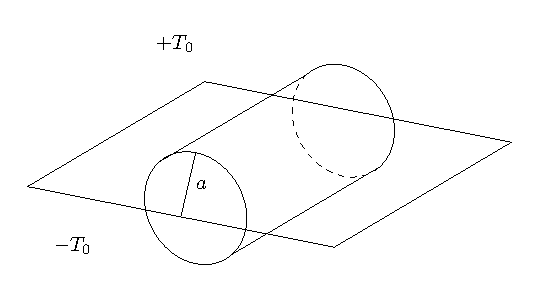
\includegraphics[scale=1.5]{Imagenes/P1_Cilindro_01.eps}
    \caption{Descripción del cilindro con las dos mitades y baños térmicos.}
    \label{fig:figura_cilindro_01}
\end{figure}
\textbf{Problema: Encuentra la temperatura tanto dentro como fuera del cilindro.}
\section{Solución.}
Debemos de comenzar considerando que la ecuación de Laplace:
\begin{align*}
\laplacian{T(\va{r})} = 0
\end{align*}
Como segunda consideración, el eje $z$ coincide con el centro del cilindro y si suponemos que éste es muy largo, resulta que la temperatura $T$ no depende de $z$, así:
\begin{align*}
\laplacian{T}_{r,\varphi} (r, \varphi) = 0
\end{align*}
Por lo que la ecuación en coordenadas cilíndricas a resolver es:
\begin{align*}
\dfrac{1}{\rho} \, \left( \pdv{\rho} \, \rho \, \pdv{T}{\rho} \right) + \dfrac{1}{\rho^{2}} \, \pdv[2]{T}{\varphi} = 0
\end{align*}
Que tiene por solución:
\begin{align*}
T = \left( A_{m} \, \rho^{m} + B_{m} \, \rho^{-m} \right) \, \big[ C_{m} \, \cos (m \varphi) + D_{m} \, \sin (m \varphi) \big] + A_{0} \,\ln (\rho) + B_{0}
\end{align*}
Siendo el siguiente paso: estudiar la solución y determinar las constantes $A_{m}, B_{m}, C_{m}, D_{m}$.

\subsection{Temperatura en el interior.}
En los puntos donde $\rho < a$, debe de converger la solución de $T$, ya que en el centro $\rho = 0$ queda incluido, para que esto se cumpla, la única manera es que los coeficientes $B_{m}$ se anulen, es decir: $B_{m} = 0$
\end{document}